\documentclass[10pt]{beamer}
\usepackage[headerslides]{umnslides}
\usepackage{tikz}
\usetikzlibrary{fit,positioning,calc,shapes,backgrounds}
\usetikzlibrary{shapes.geometric, arrows}



\graphicspath{{./figures}}
\newcommand{\commonfiles}[1]{../common/#1}
\usepackage[subpreambles=true]{standalone}

\author{Charlie Kapsiak}
\title[Single Stop Update]{RPV Single Stop Search Update}
\subtitle{Non-parametric 2D Background Estimation Using Gaussian Processes}

\begin{document}



\begin{frame}
  \maketitle
\end{frame}

\begin{frame}{Table Of Contents}
  \tableofcontents
\end{frame}

% \iffalse
%   \section{Introduction and Analysis Status}
%   \label{sec:introduction}
%   
%   \begin{frame}{Bump Hunting}
%     \begin{itemize}
%     \item One of the most common classes of searches for new physics are \textit{bump hunts}.
%     \item Given some sort of smooth description of the standard model background, look for a localized bump of excess events coming from a new physics process.
%     \item 
%     \end{itemize}
%     
%     Why bbkg est is important
%   \end{frame}
%   
%   \begin{frame}{Background Estimation Strats}
%     General types of background estimation
%   \end{frame}
%   
%   
%   \begin{frame}{Ad-Hoc}
%     Drawbacks of ad-hoc parametric
%   \end{frame}
%   
%   \begin{frame}{Glimpse of GP}
%     Introduce idea of GP
%   \end{frame}
% \fi

\section[Intro]{Introduction and Analysis Status}

\begin{frame}{Analysis Target Model}
  \begin{itemize}
  \item Searching for then production and decay of a single \stopq{} to 4 standard model quarks through an RPV coupling. 
  \item Well motivated channel to look for SUSY:
    \begin{itemize}
    \item Unexplored region of RPV parameter space
    \item Large cross section allows us to probe higher masses
    \end{itemize}
  \end{itemize}


  \begin{center}
    \graphiccite{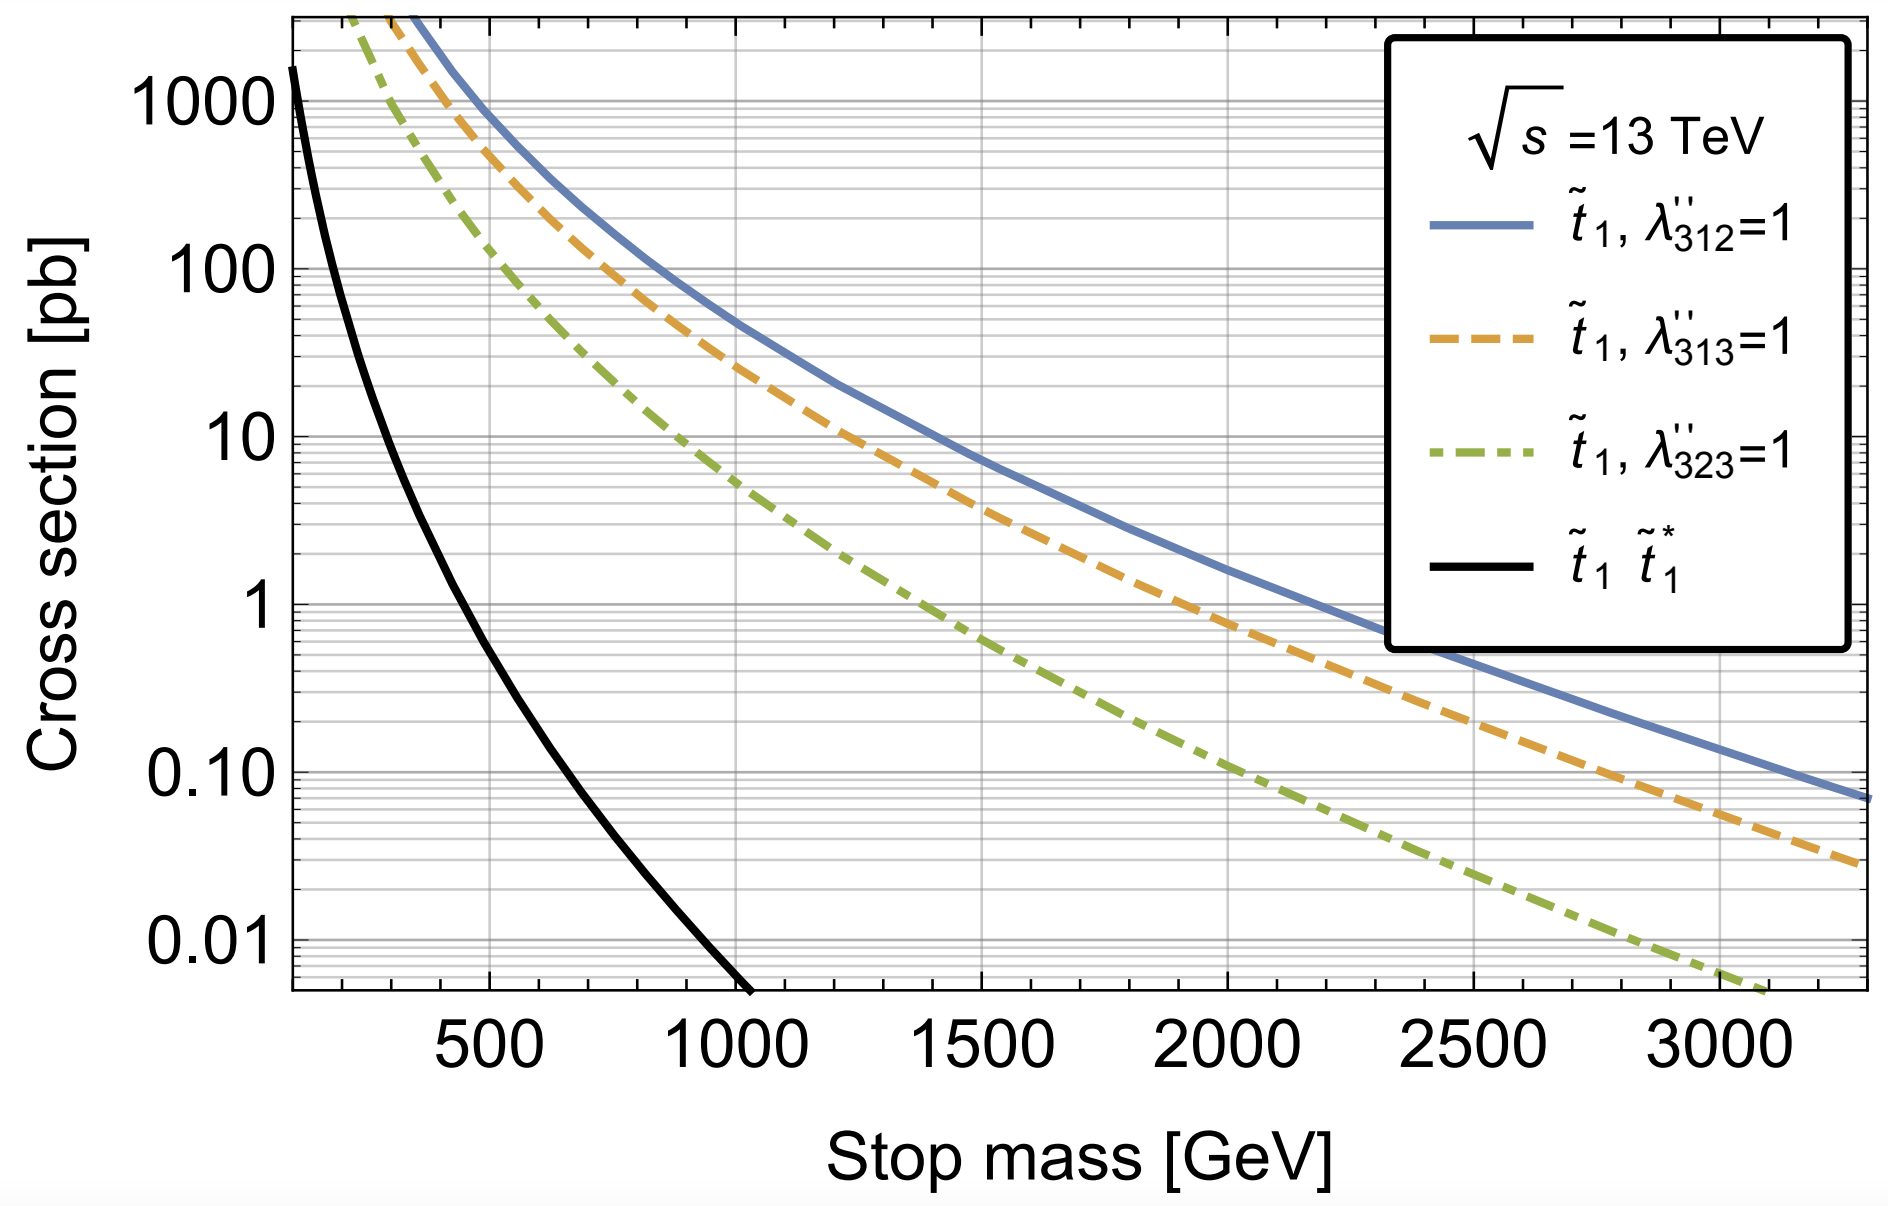
\includegraphics[width=0.5\textwidth]{figures/xsec.png}}{\cite{rasmussen_gaussian_2006}}\hspace{1em}
    \scalebox{0.7}{\includestandalone{\commonfiles{general/single_stop}}}
  \end{center}
\end{frame}


\begin{frame}{Analysis Status}
  \begin{block}{}
    The past months have seen substantial progress on several fronts. We summarize below the current major areas of work:
  \end{block}
  \begin{columns}[t]
    \begin{column}{0.5\textwidth}
      \begin{center} \textbf{Key Analysis Elements} \end{center}
      \begin{itemize}
      \coloreditem{working} Control/Signal region definitions.
      \coloreditem{working} Mass reconstruction. 
      \coloreditem{working} Background estimation
      \coloreditem{prelim} Statistical analysis procedure. 
      \coloreditem{prelim} Trigger studies.
      \coloreditem{prelim} Central MC production.
      \coloreditem{nowork} Early Run3 data.
      \end{itemize}
    \end{column}
    \begin{column}{0.5\textwidth}
      \begin{center} \textbf{Past Presentations} \end{center}
        \begin{itemize}
          \input{\commonfiles{previous_talks.tex}}
        \end{itemize}
    \end{column}
  \end{columns}

  \begin{center}
    \begin{tikzpicture}
      \path[fill=nowork] (0,0) coordinate (A) circle(0.25em);
      \node[anchor=left, right=0.1em of A] (A1) {No Work} ;

      \path[fill=prelim] ( $ (A1.east) + (0.2,0)$) coordinate (B) circle(0.25em);
      \node[anchor=left, right=0.1em of B] (B1) {Preliminary};


      \path[fill=working] ( $ (B1.east) + (0.2,0) $ ) coordinate (B) circle(0.25em);
      \node[anchor=left, right=0.1em of B] (C1) {Working Version};

      \path[fill=ready] ( $(C1.east) + (0.2,0) $) coordinate (D) circle(0.25em);
      \node[anchor=left, right=0.1em of D] {Analysis Ready};
    \end{tikzpicture}
  \end{center}
\end{frame}

\begin{frame}{General Search Strategy}
  \begin{itemize}
  \item General search strategy is to perform a one or two dimensional bump hunt for both the \stopq{} and the \chargino{} resonances. 
  \item For many mass splittings, the resonances are well separated both in $m_{\stopq, reco}$ and $m_{\chargino, reco}$ space, providing additional discriminating power.
  \item Key point is to effectively estimate the background. 
  \item However, a simple cut strategy on one mass axis can result in sculpting of the background, making estimation difficult. 
  \end{itemize}

  \begin{tikzpicture}
  \end{tikzpicture}
  \begin{center}
    \scalebox{0.5}{\includestandalone{\commonfiles{general/two_peaks}}}
  \end{center}
\end{frame}


\begin{frame}{Estimation Strategies}
  \begin{itemize}
  \item For all bump hunts, key technique is estimation of the background shape. 
  \item Traditional bump hunts have used ad-hoc functions, chosen because they approximate the observed shape. 
  \item However, this can introduce bias from the choice of function, and it has been shown that they scale poorly with increasing luminosity \cite{frate_modeling_2017}.
  \item For multidimensional searches, the problem can also be compounded by selecting a function for a potentially nontrivial 2D shape. 
  \end{itemize}

\end{frame}

\begin{frame}{Current Strategy}
  \begin{itemize}
  \item We have implemented our background estimation using Gaussian process regression \cite{rasmussen_gaussian_2006}.
  \item This is non-parametric technique that reduces bias from the choice of parametric function.
  \item It has been shown to be robust against increasing luminosity\cite{frate_modeling_2017}.
  \item It is naturally extensible to multiple dimensions.
  \item Very well studied in statistics literature, and has a large number of well established implementations \cite{gardner_gpytorch_2021}. 
  \end{itemize}
\end{frame}


\section[GP Regression]{Gaussian Process Regression Overview}
\label{sec:gauss-proc-regr}

\begin{frame}{What is a Gaussian Process?}
  \begin{definition}
    A gaussian process is a possibly infinite series of random variables, any finite subset of which is jointly gaussian.
  \end{definition}


  Generall, the random variables are indexed by real values $x$, since we are generally considering regression over $\mathbb{R}^{n}$.

  A gaussian process $f(x)$ is is completely defined by its mean and covariance
  \begin{equation}
    \begin{split}
      m(x) &= \mathbb{E} \left[ f(x) \right] \\
      k(x,x') &= \mathbb{E} \left[ \left( f(x) - m(x) \right)  \left( f(x') - m(x') \right)\right] 
    \end{split}
  \end{equation}
%   \begin{alertenv}
%     Generally $m(x)$ is assumed to be 0, since this amounts to a shift, and generally the regression deduces the posterior mean very well. 
%   \end{alertenv}
% 
%   INCLUDE IMAGE HERE SHOWING HOW 2 POINTS ARE DRAWN FROM 2D GAUSSIAN

  \begin{center}
    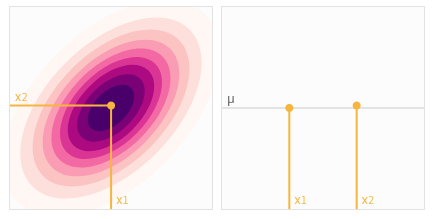
\includegraphics[width=0.4\textwidth]{figures/two_points_1}
    \hspace{1cm}
    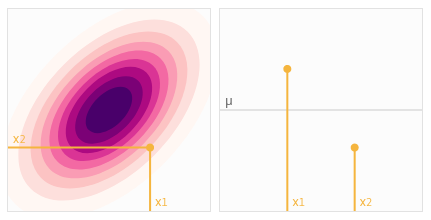
\includegraphics[width=0.4\textwidth]{figures/two_points_2}
  \end{center}
  
\end{frame}

\begin{frame}{Function Distributions}
  Gaussian process allow us to define distributions over the space of functions. Given a gaussian process $\mathcal{GP} \left( m(x) , k(x,x') \right)$, and some function $h$, then
  \begin{equation}
    \mathbf{h} \sim N(m(X) , k(X,X))
  \end{equation}
  Given $n$ points in $\mathbb{R}^{k}$, the gaussian process defined a $n$ dimensional multivariate gaussian $\mathcal{N}$. If a function $h(x)$ has has values $h_1,h_2,...,h_{n}$ at those points, then
  \begin{equation}
    p \left( h \right) \sim \mathcal{N}(h_{1}, ..., h_{n})
  \end{equation}

  \begin{center}
    \graphiccite{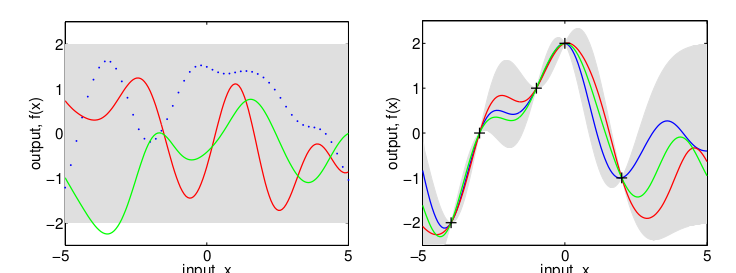
\includegraphics[width=0.7\textwidth]{figures/prior_and_conditioning}}{\cite{rasmussen_gaussian_2006}}
  \end{center}
\end{frame}

\begin{frame}{Gaussian Process Regression }
  \begin{itemize}
  \item The ability to define distributions over functions allows us to do inference using Baye's theorem. 
  \item Specifically, given $N$ training points and a Gaussian process prior, we can produce a posterior Gaussian process that provides a means to do regression. 
  \end{itemize}
  \begin{center}
    \graphiccite{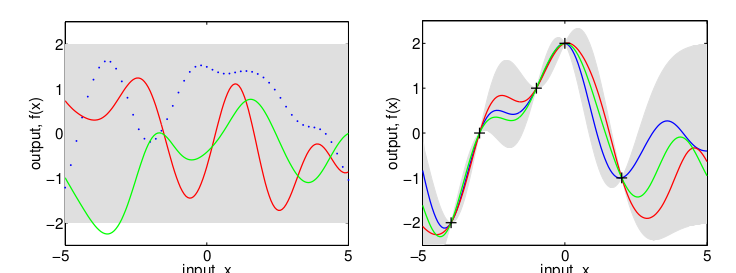
\includegraphics[width=0.7\textwidth]{figures/prior_and_conditioning}}{\cite{rasmussen_gaussian_2006}}
  \end{center}
\end{frame}

\begin{frame}{Kernels}
  \begin{itemize}
  \item The choice of kernel is the most important aspect of Gaussian processes. 
  \item Different kernels reflect different understandings of how the points should be correlated, how smooth the process the should be, etc. 
  \item There is a great deal of literature on kernels and kernel selection. Some common categories:
    \begin{itemize}
    \item Simple functions, like the square exponential or M\'atern kernel.
    \item Spectral mixtures
    \item Deep learning kernels
    \end{itemize}
  \end{itemize}

  \begin{center}
    \graphiccite{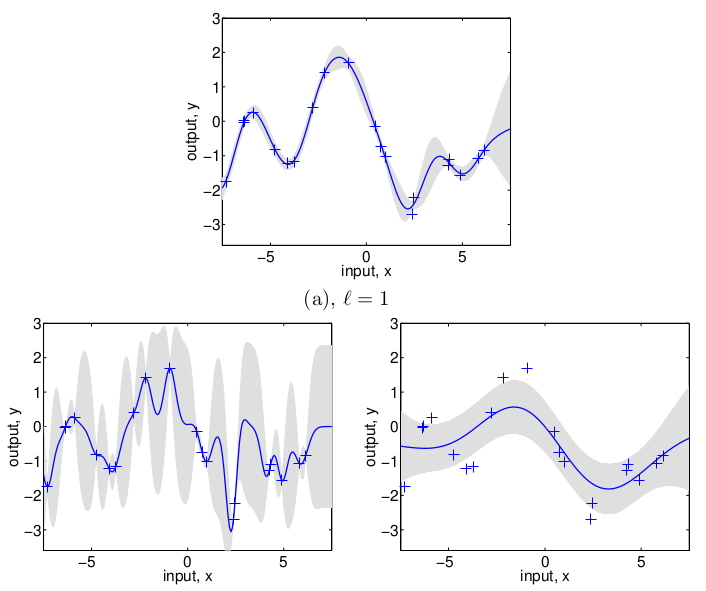
\includegraphics[width=0.4\textwidth]{figures/different_scale}}{\cite{rasmussen_gaussian_2006}}
  \end{center}
\end{frame}


\section[2D Regression]{2D Gaussian Processes and Kernels}
\label{sec:2d-gauss-proc}
\begin{frame}{Kernels}
  \begin{itemize}
  \item The machinery for Gaussian processes extends naturally to multi-dimensional problems. In our case, we examine two dimensions.
  \item In two dimenions, the kernel can have an even richer structure. 
  \end{itemize}

  \begin{center}
    \graphiccite{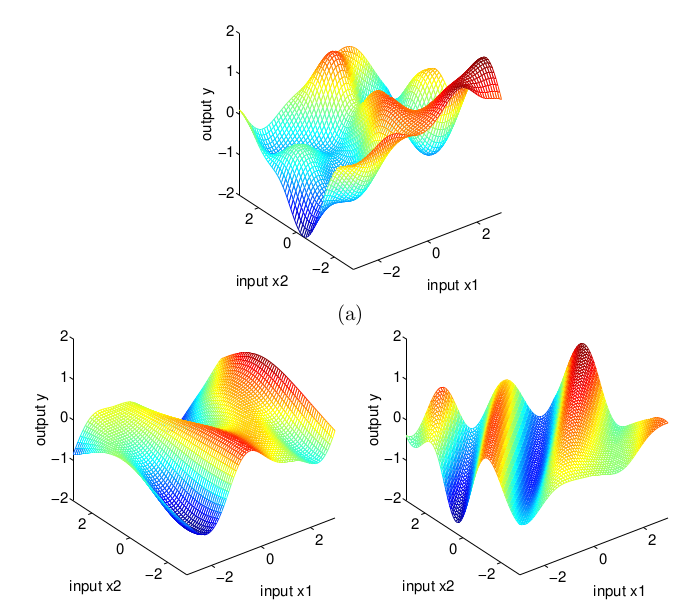
\includegraphics[width=0.4\textwidth]{figures/2d_rbf_kernels}}{\cite{rasmussen_gaussian_2006}}
  \end{center}

\end{frame}

\begin{frame}{Kernels in 2D}
  \begin{itemize}
  \item Show simplest RBF Kernel
  \item Show GRBF kernel
  \item Show NN kernel
  \end{itemize}

  SHOW IMAGES HERE OF WHAT THE DIFFERENT KERNELS LOOK LIKE
\end{frame}

\section[Results]{GP Regression for 1D and 2D Resonances}
\label{sec:results-1d-2d}

\begin{frame}{Overview}
  \begin{itemize}
  \item We use GP regression to estimate backgrounds in both one and two dimensional searches.
  \item In both cases, we mask the region of space where the signal is expected, then use regression to estimate the background in the masked region.
  \item Use both simulation and control region data to study efficacy of different methods. 
  \item Majority of studies have been focused on kernel selection and approximation techniques.
  \end{itemize}

  \begin{center}
    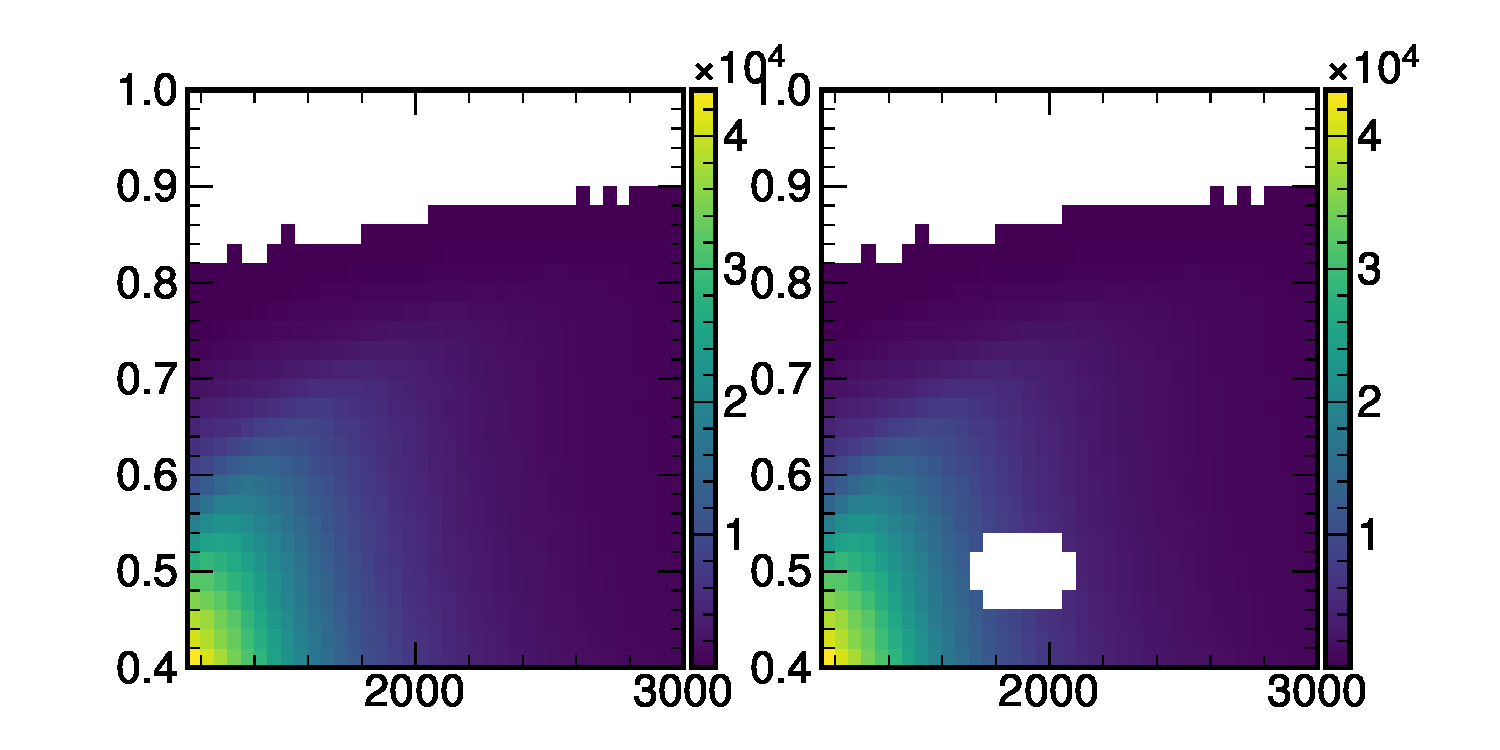
\includegraphics[width=0.7\textwidth]{figures/example_masking}
  \end{center}
\end{frame}

\begin{frame}{2D Results}
  \begin{itemize}
  \item See promising results for estimation in windows of varying sizes over the 2D plane. 
  \item Depending on region, either generalized RBF kernels or and RBF kernel supplemented with the deep network have shown promising and robust estimative abilities.
  \end{itemize}

  \begin{center}
    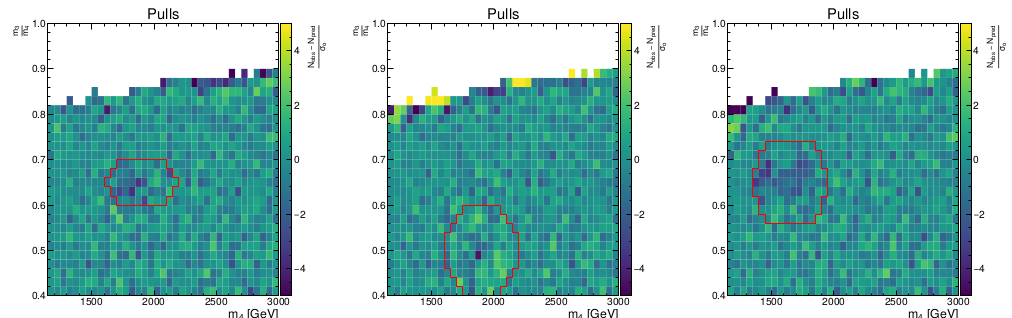
\includegraphics[width=\textwidth]{figures/nn_results_1} 
  \end{center}
\end{frame}

\begin{frame}{General RBF Fit Results}
  \begin{center}
    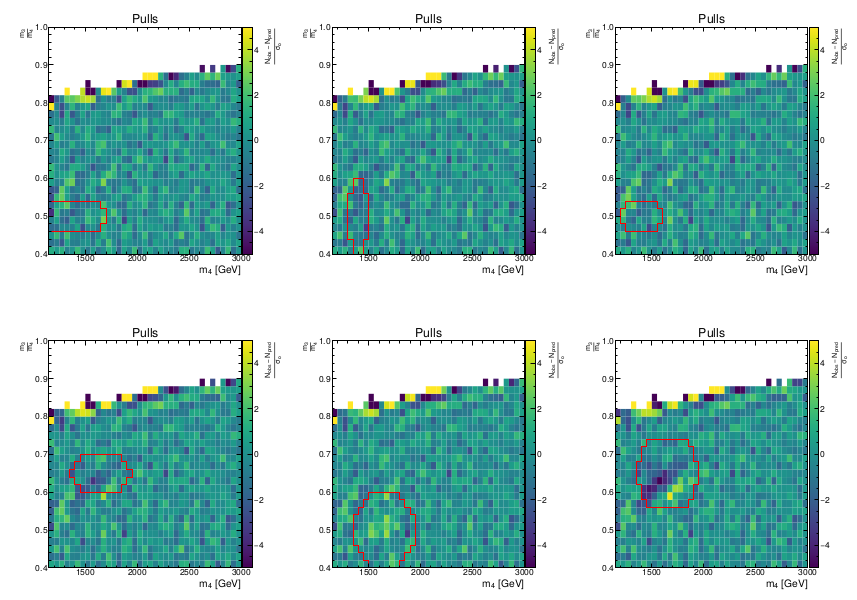
\includegraphics[width=0.9\textwidth]{figures/grbf_results} 
  \end{center}
\end{frame}

\section[Statistical Considerations]{Preliminary Statistical Strategy}

\begin{frame}{Notes on Statistical Procedure}
  \begin{itemize}
  \item Gaussian process regression provides a complete posterior distribution describing the background. 
  \item Therefore, a proper statistical treatment requires considering not just the posterior mean, but the complete distribution.
    \begin{itemize}
    \item We are working on an implementation in combine, using the eigenvectors of the posterior covariance as nuisance parameters templates. 
    \item MCMC/SVI can be externally using packages like pyro or emcee to build the statistical model directly in python.
    \end{itemize}
  \end{itemize}

  MAYBE IMAGE FROM COMBINE
\end{frame}

\begin{frame}{Systematic Uncertainties and Validation}
  \begin{itemize}
  \item We envision a validation strategy where the kernel hyperparameters are trained on SR data, then the regression is validated by examining the fit quality in simulation and CR data.
  \item More work needed to determine exactly what systematics should be considered, and how they should be implemented.
  \end{itemize}


  SHOW COMPARISON OF CR AND MC 
\end{frame}


\section{Conclusion}
\label{sec:conclusion}

\begin{frame}{Related Ongoing Work}
  \begin{itemize}
  \item Unify kernels for different mass points. We believe this will be relatively straightforward since the GRBF kernel lies in the space of deep kernels. 
  \item Finalize Combine implementation and perform validation.
  \item Work on exact definitions of systematic uncertainties.
  \item 
  \end{itemize}
  
\end{frame}

\begin{frame}{Conclusion}
  \begin{itemize}
  \item The past months have seen substantial progress on the background estimation and statistical analysis procedure.
  \item Framework can now produce good estimates for 2D backgrounds over a range of locations and masking windows.
  \item We hope to hear any feedback from experts regarding the methodology, or any comments or suggestions!
  \end{itemize}
  \vspace{1cm}

  \begin{center}
    {\Large Thank you!}
  \end{center}
\end{frame}


\begin{frame}{Bibliography}
  \bibliographystyle{plain}
  \bibliography{../bibliography.bib}
\end{frame}


\appendix

\section{Appendix}
\label{sec:appendix}


\begin{frame}{Luminosity Issues}
  \relax  
\end{frame}

\begin{frame}{Table of Common Kernels}
  \relax  
\end{frame}


\end{document}



% Local Variables:
% eval: (progn (setq process-environment (copy-sequence process-environment))
%       (let ((texmfpath (file-name-concat (file-name-directory (directory-file-name (file-name-directory (buffer-file-name)))) "texmf"))\binom{}{})
%      (setq-local TeX-style-path (append TeX-style-path  (directory-files-recursively texmfpath "auto" t)))
%      (setenv "TEXMFHOME" texmfpath )))
% End:
